\documentclass[border=6pt]{standalone}
\usepackage{amsmath}
\usepackage{amssymb}
\usepackage{tikz}
\usepackage{pgfplots}
\pgfplotsset{compat=1.18}
\usetikzlibrary{arrows.meta,calc,positioning}
\begin{document}
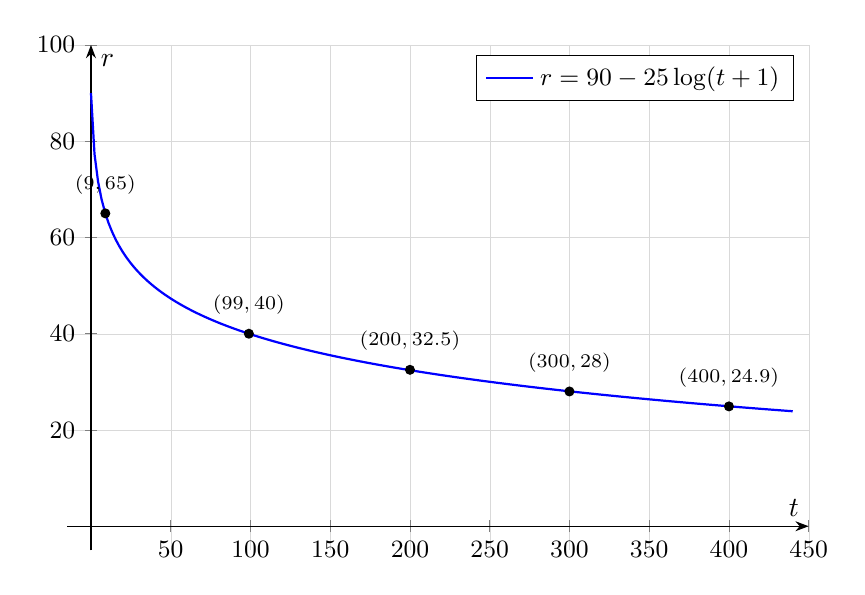
\begin{tikzpicture}
\begin{axis}[
    axis lines = middle,
    xlabel = {$t$}, ylabel = {$r$},
    grid=both,
    grid style={line width=.1pt, draw=gray!30},
    axis line style={-Stealth},
    legend style={font=\small},
    tick label style={font=\small},
    xmin=-15, xmax=450, ymin=-5, ymax=100,
    xtick={0,50,100,150,200,250,300,350,400,450},
    ytick={0,20,40,60,80,100},
    width=11cm, height=8cm,
]
\addplot[domain=0:440, samples=200, thick, blue] {90-25*(ln(x+1)/ln(10))};
\addlegendentry{$r=90-25\log(t+1)$}
\addplot[only marks, mark=*, mark size=1.6pt, black] coordinates {(9,65) (99,40) (200,32.5) (300,28) (400,24.9)};
\node[anchor=south, font=\scriptsize] at (axis cs:9,67) {$(9,65)$};
\node[anchor=south, font=\scriptsize] at (axis cs:99,42) {$(99,40)$};
\node[anchor=south, font=\scriptsize] at (axis cs:200,34.5) {$(200,32.5)$};
\node[anchor=south, font=\scriptsize] at (axis cs:300,30) {$(300,28)$};
\node[anchor=south, font=\scriptsize] at (axis cs:400,26.9) {$(400,24.9)$};
\end{axis}
\end{tikzpicture}
\end{document}
